  
\chapter{Empresa emqbit LTDA.}
\label{ap:emqbit}


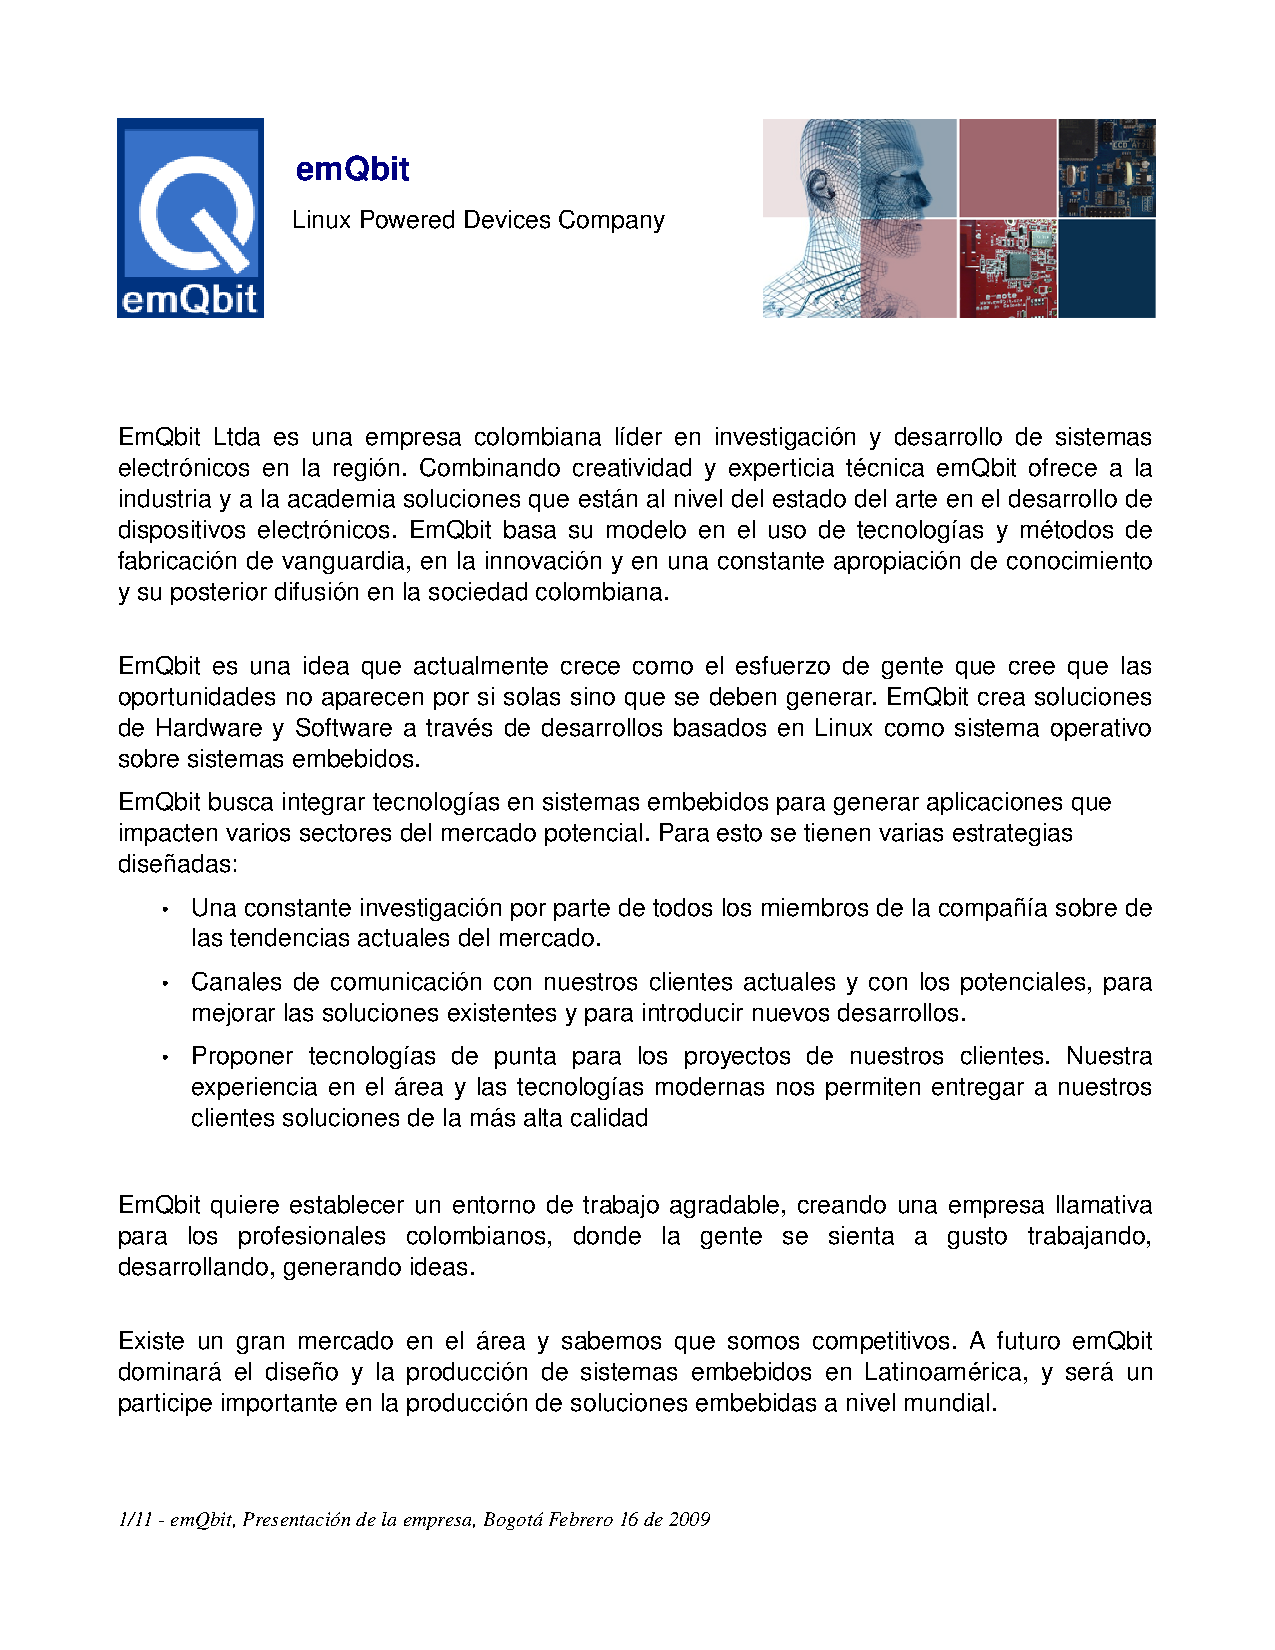
\includepdf[pages=-]{./anexos/documento_emqbit.pdf} 

\vspace{15 mm}

\begin{center} \textbf{A quien corresponda}\end{center}

\vspace{10 mm}


Como gerente general de la empresa emQbit certifico que el profesor Carlos Iv�n Camargo Bare�o ha colaborado en diversas tareas de dise�o, soporte y capacitaci�n, los productos realizados en conjunto con el profesor Camargo poseen la licencia Creative Commons BY-SA la que permite su uso, reproducci�n y modificaci�n a�n para uso comercial, con el �nico requisito de dar cr�dito al autor del trabajo original y publicar los trabajos derivados bajo la misma licencia. \\


Esta filosof�a de hardware abierto es el eje de nuestra empresa, de tal forma que la mayor parte de nuestros productos poseen la licencia CC-BY-SA; esto debido a que por un lado, gran parte de ellos se deriva de tarjetas de desarrollo elaboradas por el profesor Camargo y por otro lado, uno de los objetivos de la creaci�n de emQbit es ayudar a la difusi�n del conocimiento necesario para dise�ar e implementar sistemas digitales que utilizan tecnolog�a de punta. \\


Adicionalmente, el profesor Camargo particip� en la creaci�n de emQbit proporicionando las plataformas dise�adas por �l para que fueran utilizadas como dise�os de referencia para la creaci�n de nuevos productos, de igual forma, proporcion� soporte t�cnico para la implementaci�n de la funcionalidad requerida. \\


\begin{center}
 


\includegraphics[scale=.65]{./images/sign_afc}\\
Andr�s Felipe Calder�n de Restrepo\\
Gerente General emQbit LTDA.\\
C.C. 79.684.619 de Bogot�\\

\end{center}
